\documentclass{../notatki}

\usetikzlibrary{chains, decorations.pathreplacing}

\title{Kryptografia z elementami algebry}

\begin{document}

\tableofcontents

\section{Złożoność obliczeniowa}

\subsection{Dodawanie}

Dodanie dwóch liczb binarnych $a$ i $b$ o długości $n$ ma złożoność $O(n)$,
lub lepiej $O(\log \max(a, b))$.

\subsection{Mnożenie}

Mnożenie dwóch liczb binarnych $a$ i $b$ o długości $n$ ma złożoność $O(n^2)$,
lub lepiej $O(\log^2 \max(a, b))$.

\subsection{Potęgowanie}

Potęgowanie liczby $a$ do potęgi $b$ ma złożoność $O(\log b \log^2 a)$.

\subsection{Dzielenie}

Dzielenie liczby $a$ przez $b$ ma złożoność $O(n^2)$.

\subsection{Modulo}

Modulo liczby $a$ przez $b$ ma złożoność $O(n^2)$.

\subsection{Znajdowanie odwrotności}

To zależy od grupy, ale dla $a$ w przypadku $Z_n$ wymaga obliczenia
$n - a$, czyli $O(\log \max(a, n))$. W przypadku $Z_n^\times$ wymaga użycia
rozszerzonego algorytmu Euklidesa. Złożoność wynosi $O(\log^2 \max(a, n))$.

\section{Struktury algebraiczne}

\begin{enumerate}
  \item $\forall_{a, b \in G} a * (b * c) = (a * b) * c$
  \item $\forall_{a, b \in G} a * b = b * a$
  \item $\exists_{e \in G} \forall_{a \in G} a * e = a$
  \item $\forall_{a \in G} a^{-1} = e$
\end{enumerate}

\begin{itemize}
  \item półgrupa: 1
  \item monoid: 1, 3
  \item grupa: 1, 3, 4
  \item grupa abelowa: 1, 2, 3, 4
\end{itemize}

Zawsze istnieje tylko jeden element neutralny operacji.
Rzędem grupy jest moc zbioru $G$.

$$\varphi(n) = |\{a \in \mathbb{Z}_n : \gcd(a, n) = 1\}|$$

$$
a \in \mathbb{Z}_p^\times \rightarrow a^{-1} = a^{p-2} \mod p
$$

\subsection{Podgrupa}

Niech $H$ będzie podgrupą grupy $G$. Wtedy:
$$
\forall_{a, b \in H} a * b \in H
$$
$$
\forall_{a \in H} a^{-1} \in H
$$
Na przykład, dla $\mathbb{Z}_{10} = \{0, 1, 2, 3, 4, 5, 6, 7, 8, 9\}$,
$H = \{0, 2, 4, 6, 8\}$ jest podgrupą grupy $\mathbb{Z}_{10}$.

\subsection{Generatory}

$$
\langle g \rangle = \{g^k : k \in \mathbb{Z}\}
$$

Grupa cykliczna, to grupa, która posiada co najmniej jednoelementowy zbiór
generatorów. $\exists_{g \in G} \langle g \rangle = G$

\subsection{Warstwy}

Dla podgrupy $H$ grupy $G$, warstwą lewostronną $H$ wyznaczoną przez
$a \in G$ jest zbiór:
$$
\begin{cases}
  a + H = \{a + h : h \in H\}\\
  aH = \{ah : h \in H\}
\end{cases}
$$

Warstwy są identyczne, albo rozłączne. Warstwy $aH$ i $bH$ są sobie
równe kiedy $a^{-1}b \in H$. Suma mnogościowa
warstw jest równa grupie $G$. Indeksem podgrupy $H$ w grupie $G$ ($G
: H$) nazywamy moc zbioru warstw względem podgrupy $H$.
$$
G : H = \frac{|G|}{|H|}
$$
Rząd podgrupy $H$ jest dzielnikiem rzędu grupy $G$.

\subsection{Homomorfizmy}

$f: G \to G'$
nazywamy homomorfizmem grupy $G$ w grupę $G'$, jeśli zachodzi:
$$
f(a + b) = f(a) + f(b)
$$
$$
f(ab) = f(a)f(b)
$$

Jeśli:
\begin{itemize}
  \item $f$ jest iniekcją, to mówimy że $f$ jest monomorfizmem.
  \item $f$ jest suriekcją, to mówimy że $f$ jest epimorfizmem.
  \item $f$ jest bijekcją, to mówimy że $f$ jest izomorfizmem.
\end{itemize}

Z własności homomorfizmu wynika, że $f(e) = f(ee) = f(e)f(e) = e'$
oraz $f(a^{-1}) = f(a)^{-1}$ i $f(a)f(a^{-1}) = f(e)$.

Zbiór $Ker(f) = \{a \in G : f(a) = e'\}$ nazywamy jądrem homomorfizmu $f$.

Zbiór $Im(f) = \{f(a) : a \in G\}$ nazywamy obrazem homomorfizmu $f$.

\subsection{Symbol Lagrange'a}

Liczba $a$ w grupie $G$ jest resztą kwadratową, jeśli istnieje $b \in
G$ takie, że $a = b^2$.

Symbol Lagrange'a jest zdefiniowany następująco:
$$
\frac{a}{p} =
\begin{cases}
  1 & \text{jeśli } a \text{ jest resztą kwadratową} \\
  0 & \text{jeśli } p|a \\
  -1 & \text{jeśli } a \text{ nie jest resztą kwadratową}
\end{cases}
$$

\subsection{Ciało p-elementowe}

Dla liczby pierwszej $p$:
$$
\mathbb{F}_p = \{0, 1, \ldots, p-1\}
$$
Struktura $(\mathbb{F}_p, +_p)$ to grupa abelowa o $p$ elementach. Równocześnie
$(\mathbb{F}_p \setminus \{0\}, \cdot_p)$ jest grupą abelową. Ciałem
$p$-elementowym jest $(\mathbb{F}_p, +_p, \cdot_p)$, gdzie:
$$
\forall_{a, b, c \in \mathbb{F}_p} a (b + c) = ab + ac \land (b + c)a = ba + ca
$$

\subsection{Krzywe eliptyczne}

Dla $p > 3$, krzywą eliptyczna $E$ nad ciałem $\mathbb{F}_p$ jest dana przez:
$$
E: y^2 = x^3 + ax + b \mod p
$$
Krzywa eliptyczna musi mieć trzy pierwiastki, stąd:
$$
\Delta_E = 4a^3 + 27b^2 \mod p \neq 0
$$

Punkt $P = (x_1, y_1)$ leży na krzywej $E / \mathbb{F}_p$ (nad
$\mathbb{F}_p$), jeśli spełnia równanie:
$$
y_1^2 = x_1^3 + ax_1 + b \mod p
$$
Zatem, zbiorem wartości krzywej jest:
$$
E(\mathbb{F}_p) = \{(x, y) \in \mathbb{F}_p \times \mathbb{F}_p : y^2
= x^3 + ax + b \mod p\} \cup \{\mathcal{O}\}
$$

\subsubsection{Twierdzenie Hesse'go}

$$
\#E(\mathbb{F}_p) = p + 1 - t
$$
gdzie $t < 2\sqrt{p}$, oraz zależy od $E$. Należy wspomnieć, że $\#E$ to jej
rząd oraz ilość punktów na krzywej.

\subsubsection{Dodawanie}

Dla dwóch punktów $P = (x_1, y_1), Q = (x_2, y_2); x_1 \neq x_2$,
oraz $R = P \oplus Q = (x_3, y_3)$.
$$
\lambda = (y_2 - y_1)(x_2 - x_1)^{-1} \mod p
$$
następnie:
$$
x_3 = \lambda^2 - x_1 - x_2 \mod p
$$
$$
y_3 = \lambda(x_1 - x_3) - y_1 \mod p
$$

\subsubsection{Potęgowanie}

Dla punktu $P = (x_1, y_1), R = P \oplus P = (x_3, y_3)$.
$$
\lambda = (3x_1^2 + a)(2y_1)^{-1} \mod p
$$
następnie jak dla dodawania.

\subsubsection{Odwracanie}

$$
P = (x_1, y_1)
$$
$$P^{-1} = (x_1, -y_1)
$$

\subsubsection{Element Neutralny}

$\mathcal{O}$ nazywamy elementem neutralnym dla grupy
$(E(\mathbb{F}_p), \oplus)$.
$$
P \oplus Q = \mathcal{O} \leftrightarrow x_1 = x_2 \land y_1 = -y_2
$$
$$
P \oplus P^{-1} = \mathcal{O}
$$

\subsubsection{Generowanie krzywej}

\begin{enumerate}
  \item Generuj $k$-bitową liczbę pierwszą $p$
  \item Losuj $a, b \in \mathbb{F}_p$
  \item Oblicz $\Delta_E = 4a^3 + 27b^2$
  \item Sprawdź, czy $\Delta_E \neq 0 \mod p$, w przeciwnym razie
    \texttt{goto} 2
  \item \texttt{return} a, b, p
\end{enumerate}

\subsubsection{Generowanie punktu}

\begin{enumerate}
  \item Losuj $x \in \mathbb{F}_p$
  \item Oblicz $y^2 = x^3 + ax + b \mod p$
  \item Jeśli $\frac{y^2}{p} = -1$ \texttt{goto} 1
  \item \texttt{return} x, y
\end{enumerate}

\section{Szyfr Shannona}

Szyfr według Shannon'a jest zdefiniowany jako:
$$
\pi = (E, D) : (C, M, K)
$$
gdzie schemat szyfrujący $E$ i schemat deszyfrowania $D$ są funkcjami:
$$
E: M \times K \rightarrow C
$$
$$
D: C \times K \rightarrow M
$$

$$
D(k, E(k, m)) = m
$$

\subsection{Szyfr XOR}

$$
K = M = C = \{0, 1\}^L
$$

$$
E(m, k) = m \oplus k
$$
$$
D(c, k) = c \oplus k
$$

\subsection{Bezpieczeństwo doskonałe}

Niech $\pi$ będzie szyfrem Shannona. Rozważmy eksperyment losowy, w którym
zmienna losowa $K$ ma rozkład jednostajny nad $K$. Jeśli zachodzi:
$$
\forall_{m_0, m_1 \in M} \forall_{c \in C} P(E(k, m_0) = c) = P(E(k, m_1) = c)
$$
to mówimy, że szyfr $\pi$ jest szyfrem doskonałym.

Jeśli $\pi$ jest szyfrem doskonałym, to $|K| \ge |M|$.

\section{Problemy}

\subsection{Problem logarytmu dyskretnego (DL)}

Niech $G = \langle g \rangle$. Problemem jest znalezienie $x$
takiego, że $g^x = a$. W zależności od grupy oraz jej rozmiaru,
ten problem może być niezwykle trudny.

\begin{figure}[H]
  \centering
  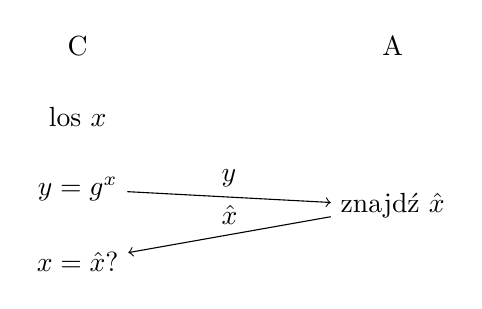
\begin{tikzpicture}[node distance=4mm]
    \node (C) at (0,0) {C};
    \node (A) at (4,0) {A};

    \begin{scope}[start chain=going below]
      \node[on chain, below=of C] (c1) {los $x$};
      \node[on chain] (c2) {$y=g^x$};
      \node[on chain] (c3) {$x=\hat{x}$?};
    \end{scope}

    \node[below=1.5cm of A] (a1) {znajdź $\hat{x}$};

    \draw[->] (c2)  -- node[midway, above] {$y$} (a1);
    \draw[->] (a1)  -- node[midway, above] {$\hat{x}$} (c3);
  \end{tikzpicture}
  \caption{Formalizm gry dla problemu logarytmu dyskretnego}
\end{figure}

\subsection{Problem DDH}

Mamy daną grupę cykliczną $G = \langle g \rangle$, rzędu
$q$, gdzie $q$ jest liczbą pierwszą. Losujemy $\alpha, \beta, \gamma
\in \mathbb{Z}_q$. Następnie obliczamy:
$$
u = g^\alpha, v = g^\beta, w_0 = g^{\alpha \beta}, w_1 = g^\gamma
$$
Celem problemu, jest odgadnięcie $b$, dla danego $u, v, w_b$.

\begin{figure}[H]
  \centering
  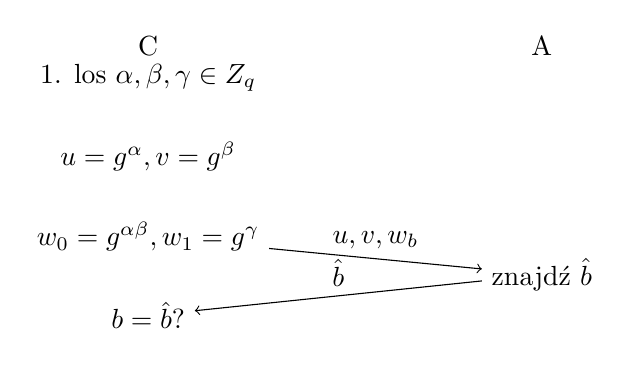
\begin{tikzpicture}[node distance=4mm]
    \node (C) at (0,0) {C};
    \node (A) at (5,0) {A};

    \begin{scope}[start chain=going below]
      \node[on chain, below of=C] (c1) {1. los $\alpha,
        \beta, \gamma \in
      \mathbb{Z}_q$};
      \node[on chain] (c2) {$u = g^\alpha, v = g^\beta$};
      \node[on chain] (c3) {$w_0 = g^{\alpha \beta}, w_1 = g^{\gamma}$};
      \node[below of=A, yshift=-2.5cm] (textA) {znajdź $\hat{b}$};
      \node[on chain] (c4) {$b = \hat{b}$?};
    \end{scope}

    \draw[->] (c3)  -- node[midway, above] {$u, v, w_b$} (textA);
    \draw[->] (textA)  -- node[midway, above] {$\hat{b}$} (c4);
  \end{tikzpicture}
  \caption{Formalizm gry dla problemu DDH}
\end{figure}

\subsection{CDH}

Mamy daną grupę cykliczną $G = \langle g \rangle$, rzędu
$q$, gdzie $q$ jest liczbą pierwszą. Losujemy $\alpha, \beta, \gamma
\in \mathbb{Z}_q$. Następnie obliczamy:
$$
u = g^\alpha, v = g^\beta, w = g^{\alpha \beta}
$$
Celem problemu, jest odgadnięcie $w$, dla danego $u, v$.

\begin{figure}[H]
  \centering
  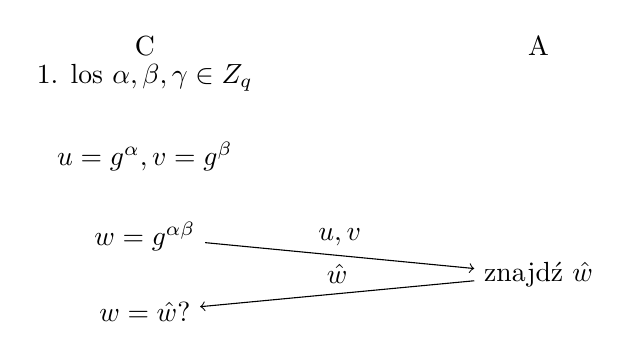
\begin{tikzpicture}[node distance=4mm]
    \node (C) at (0,0) {C};
    \node (A) at (5,0) {A};

    \begin{scope}[start chain=going below]
      \node[on chain, below of=C] (c1) {1. los $\alpha,
        \beta, \gamma \in
      \mathbb{Z}_q$};
      \node[on chain] (c2) {$u = g^\alpha, v = g^\beta$};
      \node[on chain] (c3) {$w = g^{\alpha \beta}$};
      \node[below of=A, yshift=-2.5cm] (textA) {znajdź $\hat{w}$};
      \node[on chain] (c4) {$w = \hat{w}$?};
    \end{scope}

    \draw[->] (c3)  -- node[midway, above] {$u, v$} (textA);
    \draw[->] (textA)  -- node[midway, above] {$\hat{w}$} (c4);
  \end{tikzpicture}
  \caption{Formalizm gry dla problemu CDH}
\end{figure}

\section{Schematy}

\subsection{Protokół DH}

Mamy daną grupę cykliczną $G = \langle g \rangle$, rzędu
$q$, gdzie $q$ jest liczbą pierwszą.
Protokół Diffie-Hellman (DH), polega na losowym wybraniu sekretów przez dwóch
użytkowników (A, B) $\alpha, \beta \in \mathbb{Z}_q$. Obliczeniu szyfrogramów
$u = g^\alpha, v = g^\beta$, a następnym wysłaniu $u$ i $v$. Sekret wspólny
$s = g^{\alpha \beta}$.

\begin{figure}[H]
  \centering
  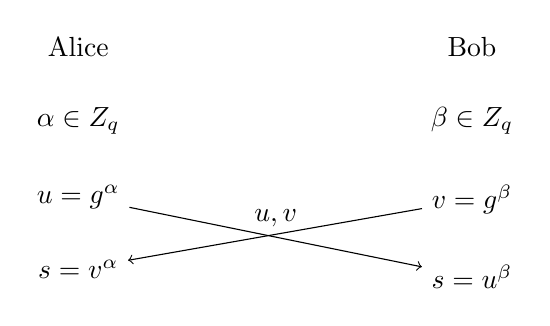
\begin{tikzpicture}[node distance=4mm]
    \node (C) at (0,0) {Alice};
    \node (A) at (5,0) {Bob};

    \begin{scope}[start chain=going below]
      \node[on chain, below=of C] (alpha) {$\alpha \in \mathbb{Z}_q$};
      \node[on chain] (u)     {$u = g^\alpha$};
      \node[on chain] (s1)     {$s = v^{\alpha}$};
    \end{scope}

    \begin{scope}[start chain=going below]
      \node[on chain, below=of A] (beta) {$\beta \in \mathbb{Z}_q$};
      \node[on chain] (v)      {$v = g^\beta$};
      \node[on chain] (s2)      {$s = u^\beta$};
    \end{scope}

    \draw[->] (u) -- node[midway, above] {$u, v$} (s2);
    \draw[->] (v) -- (s1);
  \end{tikzpicture}
  \caption{Formalizm gry dla protokołu DH}
\end{figure}

Protokół jest odporny na atak pasywny (tylko czytanie). Z kolei, jest podatny
na atak jeśli atakujący ma wpływ na kanał komunikacji, chociażby poprzez atak
Man-in-the-middle.

\subsection{Schemat szyfrowania z kluczem publicznym}

$$
\varepsilon = (G, E, D) \text{ nad } (M, C, K)
$$
gdzie $G: \mathbb{N} \to K$, $E: K \times M \to C$, $D: K \times C \to M$.

$$
(pk, sk) = G(\lambda)
$$
$$
C = E(pk, m)
$$
$$
M = D(sk, C)
$$

\section{Ataki}

\subsection{Man-in-the-middle}

Jeśli atakujący ma wplyw na kanał komunikacji, to może przechwycić komunikaty
podczas przekazywania kluczy. W takim momencie, może się podszyć pod drugą
stronę, aby uzyskać dostęp do klucza prywatnego. Równocześnie może
przekazywać dalej komunikację, aby ukryć swoją obecność. W ten sposób
zna obydwa sekrety i tylko siedzi po środku.

\subsection{Bezpieczeństwo semantyczne}

Dla pewnego $\varepsilon = (G, E, D)$, atakujący ma dostęp do klucza
publicznego $pk$. Wybiera on dwie wiadomości $m_0, m_1 \in M$. Przeciwnik
wybiera jedną wiadomość $b \in \{0, 1\}$, szyfruje ją $c = E(pk, m_b)$ i zwraca
atakującemu. Atakujący musi zgadnąć $b$.

\begin{figure}[H]
  \centering
  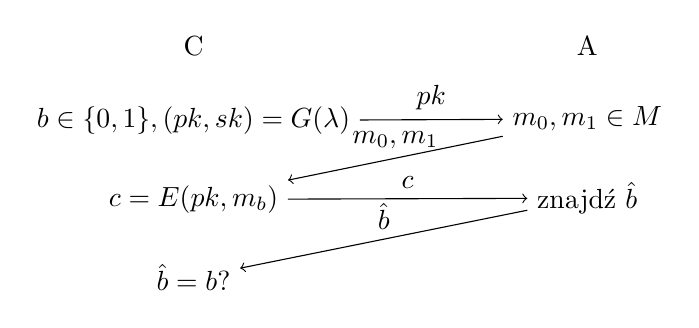
\begin{tikzpicture}[node distance=4mm]
    \node (C) at (0,0) {C};
    \node (A) at (5,0) {A};

    \begin{scope}[start chain=going below]
      \node[on chain, below=of C] (c1) {$b \in \{0, 1\}, (pk, sk) =
      G(\lambda)$};
      \node[on chain] (c2)     {$c = E(pk, m_b)$};
      \node[on chain] (c3)     {$\hat{b} = b$?};
    \end{scope}

    \begin{scope}[start chain=going below]
      \node[on chain, below=of A] (a1) {$m_0, m_1 \in M$};
      \node[on chain] (a2)      {znajdź $\hat{b}$};
    \end{scope}

    \draw[->] (c1) -- node[midway, above] {$pk$} (a1);
    \draw[->] (a1) -- node[midway, above] {$m_0, m_1$} (c2);
    \draw[->] (c2) -- node[midway, above] {$c$} (a2);
    \draw[->] (a2) -- node[midway, above] {$\hat{b}$} (c3);
  \end{tikzpicture}
  \caption{Formalizm gry dla bezpieczeństwa semantycznego}
\end{figure}

\subsection{Atak CDA}

Jest to powielona wersja bezpieczeństwa semantycznego. Wielokrotnie atakujący
może tworzyć wiadomości i dostawać losowy kryptogram na podstawie ich. To czyni
ten atak o wiele trudniejszym niż bezpieczeństwo semantyczne.

Jeśli schemat szyfrowania kluczem publicznym jest semantycznie bezpieczny,
to jest też odporny na ataki CDA.

\section{RSA}

Asymetryczny algorytm szyfrujący, w którym każda strona ma parę
kluczy: publiczny i prywatny. Enkrypcja odbywa się przy pomocy klucza
publicznego drugiej strony, a dekrypcja przy pomocy klucza prywatnego.

\subsection{Definicja}

Dla danych liczb pierwszych $p$ i $q$.

$$
n = pq
$$
$$
\varphi(n) = (p-1)(q-1)
$$
Następnie wybieramy liczbę $e$ względnie pierwszą z $\varphi(n)$.
Klucz prywatny $d$ musi spełniać warunek $ed \equiv 1
\pmod{\varphi(n)}$, zatem
$$
d = e^{-1} \pmod{\varphi(n)}
$$
$(n, e)$ tworzy klucz publiczny, a $(n, d)$ klucz prywatny.

Szyfrowanie wiadomości $M$ odbywa się za pomocą wzoru:
$$
C = M^e \pmod{n}
$$
Odkrycie wiadomości $M$ odbywa się za pomocą wzoru:
$$
M = C^d \pmod{n}
$$

\subsection{Trudność problemu}

Trudność wynika ze znalezienia $\varphi(n)$, a ponieważ weryfikacja
czy znalezione $\varphi(n)$ jest poprawne wymaga zastosowania rozszerzonego
algorytmu Euklidesa; odszyfrowanie wiadomości $C$ wymaga znalezienia $d$.

\subsection{Przykład}

$$
p = 7, q = 11 \Rightarrow n = 77, \varphi(n) = 60
$$
$$
e = 13 \Rightarrow d = 37 \Rightarrow
\begin{cases}
  (n, e) = (77, 13) \\
  (n, d) = (77, 37)
\end{cases}
$$

$$
M = 15 \Rightarrow C = 15^{13} \pmod{77} = 64
$$
$$
C = 64 \Rightarrow M = 64^{37} \pmod{77} = 15
$$

\section{Funkcja Hashująca}

$$
H: X \to Y
$$
gdzie $|X| > |Y|$. Można interpretować jako funkcję jednokierunkową, bez
zapadki. Mówimy, że $H$ jest złamana, jeśli łatwo można znaleźć
przykłady $m_0 \neq m_1$, takie że zachodzi $H(m_0) = H(m_1)$.

\section{ElGamal}

Dla grupy cyklicznej $G$ rzędu $q$, wykonujemy najpierw protokoł DH, a następnie
szyfrowanie wiadomości $m$ przy pomocy ustalonego sekretu $k$ oraz
algorytmu $(E, D)$. Zazwyczaj stosuje
się dodatkowo funkcje haszującą $H: G \times G \to K$ do generowania $k$:
$$
s = g^{\alpha\beta} \pmod{q}
$$
$$
k = H(u, s)
$$
$$
c = E(m, k)
$$
$$
m = D(c, k)
$$
Jeśli $H$ jest "dobry", czyli deterministyczny, lecz zbliżony do
losowej funkcji, oraz problem CDH jest trudny, to ElGamal jest bezpieczny.

\section{Protokół OT}

Protokół OT, pozwala na przekazanie informacji bezpiecznie, bez serwera
wiedzącego o zawartości wiadomości zwrotnej.

\begin{figure}[H]
  \centering
  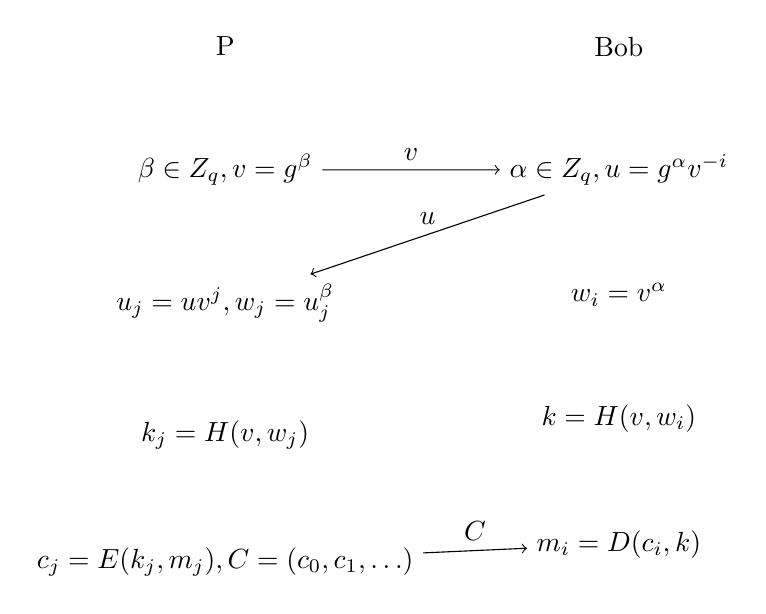
\begin{tikzpicture}
    \node (C) at (0,0) {P};
    \node (A) at (5,0) {Bob};

    \begin{scope}[start chain=going below]
      \node[on chain, below=of C] (c1) {$\beta \in \mathbb{Z}_q, v = g^\beta$};
      \node[on chain] (c2)     {$u_j = uv^j, w_j = u_j^\beta$};
      \node[on chain] (c3)     {$k_j = H(v, w_j)$};
      \node[on chain] (c4)     {$c_j = E(k_j, m_j), C=(c_0, c_1, \dots)$};
    \end{scope}

    \begin{scope}[start chain=going below]
      \node[on chain, below=of A] (a1) {$\alpha \in \mathbb{Z}_q, u =
      g^\alpha v^{-i}$};
      \node[on chain] (a2)      {$w_i = v^\alpha$};
      \node[on chain] (a3)      {$k = H(v, w_i)$};
      \node[on chain] (a4)      {$m_i = D(c_i, k)$};
    \end{scope}

    \draw[->] (c1) -- node[midway, above] {$v$} (a1);
    \draw[->] (a1) -- node[midway, above] {$u$} (c2);
    \draw[->] (c4) -- node[midway, above] {$C$} (a4);
  \end{tikzpicture}
  \caption{Schemat protokołu}
\end{figure}

$$
w_i = u_i^\beta = (uv^i)^\beta = (g^\alpha v^{-i} v^{i})^\beta =
g^{\alpha \beta}
$$

\section{Szyfry blokowe}

Szyfrem blokowym, nazywamy szyfr, który szyfruje blok bitów wejściowych
w blok równej długości, uznawany za szyfrogram.
$$
E: M \rightarrow M, D: M \rightarrow M
$$

\subsection{Bezpieczeństwo}

Klasę permutacji, na zbiorze $X$, będziemy nazywać $Perms(X)$

\begin{figure}[H]
  \centering
  \begin{tikzpicture}
    \node (C) at (0,0) {C};
    \node (A) at (5,0) {A};

    \begin{scope}[start chain=going below]
      \node[on chain, below=of C] (c1) {$b \in \{0, 1\}$};
      \node[on chain] (c2)     {$f = E(k, \dots) : b = 0 \vee f \in
      Perms(X) : b = 1$};
      \node[on chain] (c3)     {$y_i = f(x_i)$};
      \node[on chain] (c4)     {$b = \hat{b}$?};
    \end{scope}

    \begin{scope}[start chain=going below]
      \node[on chain, below=of A] (a1) {};
      \node[on chain] (a2)     {};
      \node[on chain] (a3)      {$x_1, x_2, \dots, x_n \in X$};
      \node[on chain] (a4)      {znajduje $\hat{b} \sim b$};
    \end{scope}

    \draw[->] (a3) -- node[midway, above] {$x_i$} (c3);
    \draw[->] (c3) -- node[midway, above] {$y_i$} (a4);
    \draw[->] (a4) -- node[midway, above] {$\hat{b}$} (c4);
  \end{tikzpicture}
  \caption{Gra określająca bezpieczeństwo szyfru blokowego}
\end{figure}

Szyfr blokowy jest bezpieczny, jeśli $P(b = \hat{b}) \approx 1/2$

\subsection{Nieprzewidywalność}

\begin{figure}[H]
  \centering
  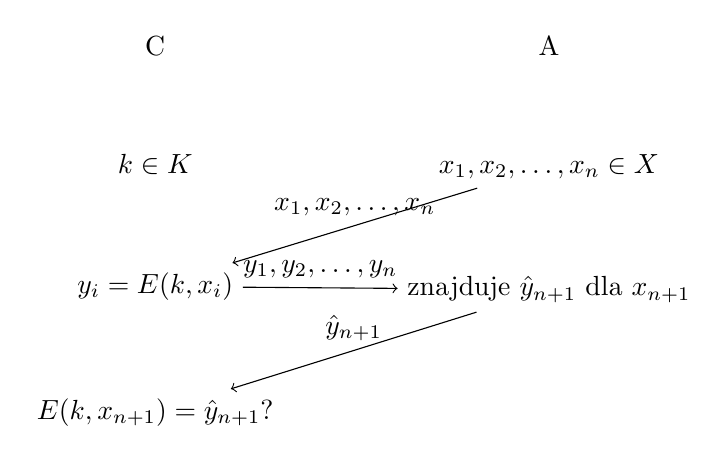
\begin{tikzpicture}
    \node (C) at (0,0) {C};
    \node (A) at (5,0) {A};

    \begin{scope}[start chain=going below]
      \node[on chain, below=of C] (c1) {$k \in K$};
      \node[on chain] (c2)     {$y_i = E(k, x_i)$};
      \node[on chain] (c3)     {$E(k, x_{n + 1}) = \hat{y}_{n+1}$?};
    \end{scope}

    \begin{scope}[start chain=going below]
      \node[on chain, below=of A] (a1) {$x_1, x_2, \dots, x_n \in X$};
      \node[on chain] (a2)      {znajduje $\hat{y}_{n+1}$ dla $x_{n+1}$};

    \end{scope}

    \draw[->] (a1) -- node[midway, above] {$x_1, x_2, \dots, x_n$} (c2);
    \draw[->] (c2) -- node[midway, above] {$y_1, y_2, \dots, y_n$} (a2);
    \draw[->] (a2) -- node[midway, above] {$\hat{y}_{n+1}$} (c3);
  \end{tikzpicture}
  \caption{Gra określająca nieprzewidywalność szyfru blokowego}
\end{figure}

Jeśli szyfr blokowy jest bezpieczny, to nieprzewidywalność jest spełniona.
Jeśli szyfr jest przewidywalny, to nie może być bezpieczny, ponieważ mogąc
przewidzieć $\hat{y}$, możemy łatwo porównać czy $\hat{y} = E(k, x_{n+1})$.

\subsection{Odzyskanie klucza}

\begin{figure}[H]
  \centering
  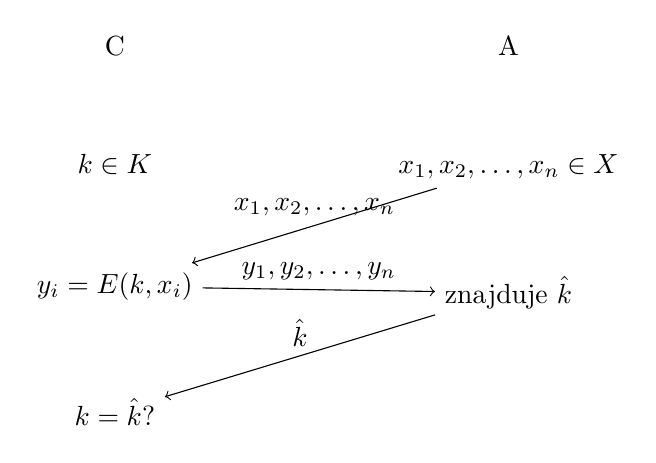
\begin{tikzpicture}
    \node (C) at (0,0) {C};
    \node (A) at (5,0) {A};

    \begin{scope}[start chain=going below]
      \node[on chain, below=of C] (c1) {$k \in K$};
      \node[on chain] (c2)     {$y_i = E(k, x_i)$};
      \node[on chain] (c3)     {$k = \hat{k}$?};
    \end{scope}

    \begin{scope}[start chain=going below]
      \node[on chain, below=of A] (a1) {$x_1, x_2, \dots, x_n \in X$};
      \node[on chain] (a2)      {znajduje $\hat{k}$};

    \end{scope}

    \draw[->] (a1) -- node[midway, above] {$x_1, x_2, \dots, x_n$} (c2);
    \draw[->] (c2) -- node[midway, above] {$y_1, y_2, \dots, y_n$} (a2);
    \draw[->] (a2) -- node[midway, above] {$\hat{k}$} (c3);
  \end{tikzpicture}
  \caption{Gra określająca odzyskanie klucza szyfru blokowego}
\end{figure}

Jeśli $E$ jest nieprzewidywalny, to jest odporny na odzyskiwanie klucza.

\subsection{DES}

DES (Data Encryption Standard) to archetypiczny szyfr blokowy. Transformuje on,
albowiem pewien blok bitów (64) w blok równej długości, uznawany za szyfrogram.
DES używa klucza długości 64 bitów, ale jedynie 56 bitów jest używanych do
szyfrowania.

Deszyfrowanie składa się z tej samej serii operacji, jedynie z kluczami
używanymi w odwrotnej kolejności. To oznacza, że wystarczy jedna implementacja
sprzętowa szyfrowania.

\subsubsection{Enkrypcja}

DES składa się z 16 rund, poprzedzonych permutacją wejściową ($IP$),
oraz zakończoną permutacją wyjściową ($FP = IP^{-1}$). Blok wejściowy
jest dzielony na pół, i operacje są wykonywane na obu częściach na przemian.
$F(S)$ oznacza funkcję szyfrowania, dla klucza 48 bitowego $S$.

\begin{figure}[H]
  \centering
  \begin{tikzpicture}
    \node[draw, rectangle, minimum width=8cm, minimum height=1cm]
    (input) {$IP$};

    \coordinate (BL) at (input.south west);
    \coordinate (BM) at ($(input.south west)!0.5!(input.south east)$);
    \coordinate (BR) at (input.south east);

    % points slightly below the box for the horizontal bracket segment
    \coordinate (BLM) at ($(BL)!0.5!(BM)+(0,-4mm)$);
    \coordinate (BRM) at ($(BM)!0.5!(BR)+(0,-4mm)$);

    \draw[line width=0.4pt]
    (BL) -- (BLM)
    -- (BM);

    \draw[line width=0.4pt]
    (BM) -- (BRM)
    -- (BR);

    \node[draw, rectangle, minimum width=1.5cm, minimum height=1cm,
    below=of BM] (F_1) {$F(K_1)$};
    \node[left=of F_1] (xor_1) {$\oplus$};
    \node[right=of F_1] (nil_1) {};

    \node[draw, rectangle, minimum width=1.5cm, minimum
    height=1cm, below=of F_1] (F_2) {$F(K_2)$};
    \node[right=of F_2] (xor_2) {$\oplus$};
    \node[left=of F_2] (nil_2) {};

    \node[below=of F_2] (dots) {$\dots$};

    \draw[->] (F_1) -- (xor_1);
    \draw[->] (BLM) -- (xor_1);
    \draw[->] (BRM) -- (xor_2);
    \draw[->] (nil_1) -- (F_1);

    \node[draw, rectangle, minimum width=8cm, minimum height=1cm, below=of dots]
    (fp) {$FP$};

    \coordinate (BL) at (fp.north west);
    \coordinate (BM) at ($(fp.north west)!0.5!(fp.north east)$);
    \coordinate (BR) at (fp.north east);

    \coordinate (BLM) at ($(BL)!0.5!(BM)+(0,+4mm)$);
    \coordinate (BRM) at ($(BM)!0.5!(BR)+(0,+4mm)$);

    \draw[line width=0.4pt]
    (BL) -- (BLM)
    -- (BM);

    \draw[line width=0.4pt]
    (BM) -- (BRM)
    -- (BR);

    \draw[->] (F_2) -- (xor_2);
    \draw[->] (xor_1) -- (BLM);
    \draw[->] (nil_2) -- (F_2);
    \draw[->] (xor_2) -- (BRM);

  \end{tikzpicture}
  \caption{Schemat szyfrowania DES}
\end{figure}

\subsubsection{Generowanie kluczy}

Generowanie kluczy $S_n$ polega na kolejnych transformacji połówek
klucza początkowego $K$. Najpierw klucz $K$ jest transformowany przez
permutację $PC1$ do 56 bitów i dzielony na dwie 28-bitowe połowy $L_0$ i $R_0$.
Następnie $L_0$ i $R_0$ są przesuwane o $p(n)$ bitów w lewo, gdzie $p(n)$
jest zależne od rundy $n$. Po przesunięciu, $L_n$ i $R_n$ są
połączone i permutowane przez $PC2$ do 48 bitów, aby uzyskać klucz
$K_n$. Generacja $K_n = PC2(L_{n - 1} << p(n) | R_{n - 1} << p(n))$.
Do dekrypcji, używamy kluczy $K_n$ w odwrotnej kolejności, zatem najpierw
$K_{16}$, a następnie $K_{15}$, itd.

\subsubsection{Funkcja F (Feistel)}

Najpierw nasze 32 bity wejściowe szyfrogramu $C$ są poddawane transformacji $E$
do 48 bitów ($4 \cdot 6$). Następnie szyfrogram jest mieszany z
kluczem, zatem $I = E(C) \oplus K_n$. Po tym, $I$
jest dzielone na 8 bloków po 6 bitów ($I_1, I_2, \ldots, I_8$), które
są przekazywane do odpowiednich S-boxów. S-boxy działają jak funkcje
nieliniowe i stanowią główne źródło bezpieczeństwa DES. Wyniki działania są
transformowane przez $P$, dzięki czemu bity są równo dystrybuowane po
całym 32-bitowym wyjściu.

$$
I = E(C) \oplus K_n
$$
$$
F(K_n) = P(S_1(I_1) | S_2(I_2) | \ldots | S_8(I_8))
$$

\subsubsection{Permutacja E}

\begin{figure}[H]
  \centering
  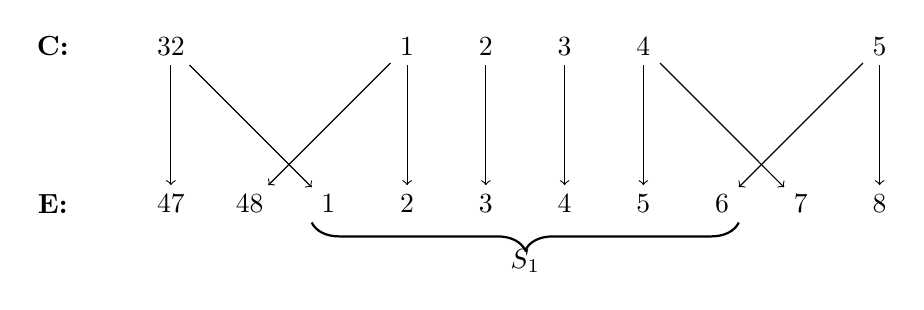
\begin{tikzpicture}

    \node (label1) at (-1.5,0) {\textbf{C:}};

    \node (a1) at (0,0) {32};
    \node (a2) at (3,0) {1};
    \node (a3) at (4,0) {2};
    \node (a4) at (5,0) {3};
    \node (a5) at (6,0) {4};
    \node (a6) at (9, 0) {5};

    \node (label2) at (-1.5,-2) {\textbf{E:}};

    \node (b1) at (0,-2) {47};
    \node (b2) at (1,-2) {48};
    \node (b3) at (2,-2) {1};
    \node (b4) at (3,-2) {2};
    \node (b5) at (4,-2) {3};
    \node (b6) at (5,-2) {4};
    \node (b7) at (6,-2) {5};
    \node (b8) at (7,-2) {6};
    \node (b9) at (8,-2) {7};
    \node (b10) at (9,-2) {8};

    \draw[->] (a1) -- (b1);
    \draw[->] (a1) -- (b3);
    \draw[->] (a2) -- (b2);
    \draw[->] (a2) -- (b4);

    \draw[->] (a3) -- (b5);
    \draw[->] (a4) -- (b6);
    \draw[->] (a5) -- (b7);
    \draw[->] (a5) -- (b9);
    \draw[->] (a6) -- (b8);
    \draw[->] (a6) -- (b10);

    \draw[decorate,decoration={brace,amplitude=10pt,mirror},thick]
    (b3.south west) -- (b8.south east)
    node[midway,yshift=-14pt,draw=none,fill=none] {$S_1$};
  \end{tikzpicture}
  \caption{Permutacja E}
\end{figure}

\subsubsection{S-Boxy}

S-Boxy, to funkcje nieliniowe, mające zapewnić większy poziom
bezpieczeństwa DES. Są one definiowane przez tablicę $16 \times 4$.
Indeksowana jest przez $x$ i $y$, gdzie $x \in \{0, 1, \ldots, 15\}$
i $y \in \{0, 1, 2, 3\}$, wyciągane z sześciu bitów wejścia.
\begin{figure}[H]
  \centering
  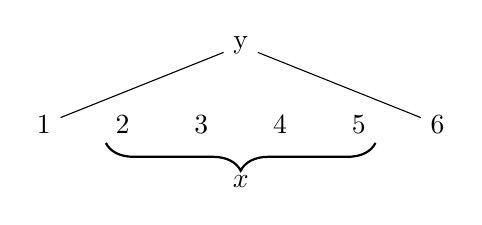
\begin{tikzpicture}
    \node(y) at (4.5, 0) {y};

    \node (a) at (2,-1) {1};
    \node (b) at (3,-1) {2};
    \node (c) at (4,-1) {3};
    \node (d) at (5,-1) {4};
    \node (e) at (6,-1) {5};
    \node (f) at (7,-1) {6};

    \draw[decorate,decoration={brace,amplitude=10pt,mirror},thick]
    (b.south west) -- (e.south east)
    node[midway,yshift=-14pt,draw=none,fill=none] {$x$};

    \draw[-] (a) -- (y);
    \draw[-] (f) -- (y);
  \end{tikzpicture}
  \caption{Ilustracja interpretacji wejścia do S-Boxa jako koordynaty $(x,y)$}
\end{figure}

Założeniem S-boxa, jest zapewnienie tego, że zmiana jednego bitu
wejścia zapewnia \textbf{co najmniej} zmianę dwóch bitów wyjścia. To oznacza, że
ilość bitów zmienionych przez S-box jest \textbf{co najmniej} równa $2$ i
potrzeba maksymalnie 6 rund aby zmiana jednego bitu wpłynęła na całe wyjście.

\subsubsection{Bezpieczeństwo}

DES nie jest bezpieczny na dwóch frontach: jego wielkość klucza i jego własności
kryptoanalityzcne.

64 bitowy klucz to po prostu za mało, zwłascza, że tak naprawdę
klucz ma 56 bitów. Klucz DES mieści się w jednym rejestrze w
architekturach 64-bitowych i przeszukanie wszystkich kluczy wiąże się
z jedną pętlą \texttt{for} na type \texttt{uint64\_t}. \textit{Notka
od autora:} założyłem się z wykładowcą, czy
taki atak jest praktyczny. Iteracja po 40 bitach klucza przy pomocy instrukcji
\texttt{avx512} zajmuje około 8.6s. To oznacza, że iteracja po 56 bitach powinna
zająć około 6.5 dnia.

Bardziej zaawansowane ataki, opierające się na kryptoanalizie potrafią rozwiązać
problem CDA w $2^{50}$ rund z prawdopodobieństwem $50\%$.

\subsubsection{Whitening}

Poziom bezpieczeństwa DES można poprawić poprzez dodanie dodatkowego klucza
do każdego bloku danych. Ten dodatkowy klucz jest używany do $\oplus$ z każdym
blokiem danych przed szyfrowaniem.

\end{document}
